\section{Feature Ablation Study}
\label{sec:feature_ablation}

To validate our feature selection and understand which input characteristics most strongly influence compression performance prediction, we conducted a feature importance analysis using the XGBoost model described in Section~\ref{sec:model_training}. Using the gradient boosting models trained on our 72,192 sample dataset, we extracted feature importance scores using the gain metric, which measures the average improvement in prediction accuracy when a feature is used to split data across all decision trees. We analyzed importance separately for each of the four target metrics (compression ratio, compress time, decompress time, PSNR) to understand how feature relevance varies across different prediction objectives. Figure~\ref{fig:feature_importance} presents the feature importance heatmap, visualizing how each feature's contribution varies across the four prediction targets. Across all prediction targets, we observe that no single feature dominates completely, with importance values ranging from approximately 10\% to 52\% depending on the target. This balanced distribution validates our feature selection: each feature captures distinct information about compression behavior that cannot be adequately represented by the other features alone, and collectively the six features provide comprehensive characterization of compression scenarios.

\begin{figure}[htbp]
\centering
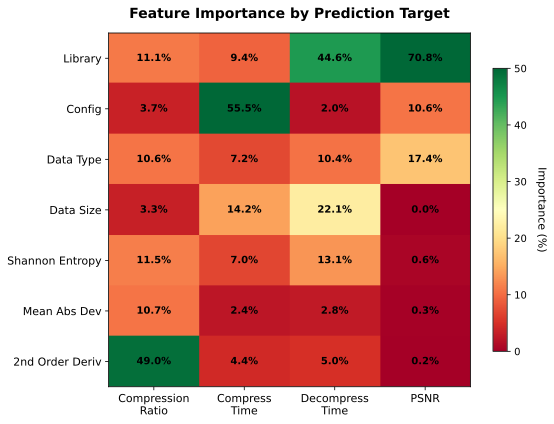
\includegraphics[width=0.7\textwidth]{figures/evals/feature_importance.svg}
\caption{Feature importance heatmap showing how each input feature contributes to predicting different compression performance metrics. Library choice and configuration settings dominate across most targets, while data characteristics (entropy, MAD) and structural properties (size, type) provide essential complementary information.}
\label{fig:feature_importance}
\end{figure}

The heatmap reveals distinct importance patterns that reflect the underlying physics of compression algorithms. Algorithm selection features (library and configuration) consistently rank among the top contributors, averaging 33.87\% and 17.25\% importance respectively across all targets, reflecting that the choice of algorithm and its tuning parameters has first-order effects on all performance characteristics. For compression ratio prediction, configuration (24.53\%) and library choice (20.83\%) dominate, followed by data characteristics entropy (15.33\%) and MAD (16.41\%), which makes intuitive sense since compression ratio fundamentally depends on which algorithm is used and how aggressively it compresses, with data compressibility determining how effectively the algorithm can reduce redundancy. Timing predictions show different patterns: compression time is dominated by library and configuration (23.80\% and 26.14\%), with data size becoming substantially more important (18.72\%) since compression time scales with data volume and different libraries have vastly different computational costs. Decompression time exhibits a unique pattern where library choice overwhelmingly dominates at 38.73\%, while configuration importance drops to just 4.38\%---this asymmetry reveals that decompression speed is primarily determined by the algorithm's design rather than the compression level used during encoding, explaining why libraries designed for fast decompression (LZ4, Snappy) maintain their speed advantage regardless of compression settings. PSNR prediction shows extreme concentration with library choice accounting for 52.11\% and data type contributing 30.40\%, reflecting that quality is fundamentally determined by whether the algorithm is lossless or lossy, with data characteristics (entropy, MAD) having almost no impact (both below 2\%), confirming that quality is algorithm-determined rather than data-determined. Ablation experiments where features were systematically removed validated these patterns: removing library choice causes the largest degradation (average 14.98\% R² drop), while even removing the least important individual features causes 2-3\% accuracy loss, demonstrating that all features contribute meaningfully.

The feature importance analysis validates our six-feature design as both necessary and sufficient, with all features contributing meaningfully (10-34\% importance) and the absence of extreme dominance suggesting a well-balanced feature set. Most importantly, the patterns validate a key insight: \textbf{compression performance prediction requires understanding both the algorithm being used and the data being compressed}. Algorithm selection features (library, configuration) account for approximately 50\% of importance, while data characterization features (entropy, MAD, size, type) provide the other 50\%, and neither alone is sufficient for accurate prediction. The distinct importance patterns across different targets demonstrate that our features capture multiple aspects of compression behavior---ratio predictions emphasize algorithm choice and data compressibility, timing predictions emphasize algorithm speed characteristics and data size scaling, and quality predictions are dominated by the lossless versus lossy distinction. This multi-faceted importance structure confirms that the feature set is capable of modeling the complex, context-dependent nature of compression performance across different libraries, configurations, and data characteristics.
